\documentclass[11pt]{article}
\pdfinfoomitdate=1\pdftrailerid{}
\usepackage[letterpaper,margin=.7in,headheight=15pt,headsep=18pt,footskip=24pt]{geometry}
\usepackage[T1]{fontenc}\usepackage{lmodern,amsmath,amssymb,array,booktabs,fancyhdr,needspace,hyperref,tikz,enumitem}
\renewcommand{\familydefault}{\sfdefault}\setlength{\parindent}{0pt}\setlength{\parskip}{6pt}
\pagestyle{fancy}\fancyhf{}\fancyhead[L]{\small Week NN / Towers from either end / Facilitator guide}
\fancyfoot[L]{\scriptsize Bellingham Math Circle / Week NN / NN-FAC-v1}\fancyfoot[R]{\thepage}
\renewcommand{\headrulewidth}{0.4pt}
\hypersetup{colorlinks=false,pdfborder={0 0 0}}
\definecolor{slotred}{RGB}{248,182,182}
\definecolor{slotblue}{RGB}{112,152,228}
\newcommand{\head}[1]{\par\Needspace{6\baselineskip}\medskip\textbf{\large #1}\par}
\newcommand{\sub}[1]{\par\textbf{#1}\par}
\newcommand{\pr}[2]{\par\textbf{Problem #1, page #2.}\ }

% launch picture helpers (x = 1mm)
\newcommand{\slots}[2]{% #1 = x origin, #2 = number of slots
  \foreach \i in {1,...,#2}{\draw[thick,fill=white] ({#1+(\i-1)*7},0) rectangle ++(7,4);
    \node[font=\scriptsize] at ({#1+(\i-1)*7+3.5},2) {\i};}}
\newcommand{\tower}[3]{% #1 = x center, #2 = base y, #3 = height
  \foreach \k in {1,...,#3}{\draw[fill=black!14] ({#1-1.75},{#2+(\k-1)*3.5}) rectangle ++(3.5,3.5);}}
\begin{document}
\head{Mathematical overview: on even rows a coloring guarantees the first player a tie or better; best play needs working backward}
\textbf{The game and its assumptions.} A row of towers stands in numbered slots. Two players alternate; a move removes one whole tower from either end of the row. When the row is empty the player with more cubes wins, and equal totals tie. The pages use heights 1 to 6 (1 to 5 in K--1); the theorems below hold for any heights. \emph{Playing as well as you can} means collecting as many cubes as you can be sure of, as the 2--3 and 4--5 pages define it. Scores are first player--second player under that assumption unless stated. Shade the slots alternately red and blue, slot 1 red; the \emph{red total} is the cubes on red slots.

\textbf{Theorem 1 (even rows): the first player can take every tower of either color, so never loses.} With an even number of towers the two end slots have different colors. The first player takes the end of the chosen color. Both ends of what remains are now the other color, so the opponent must take a tower of that color, and doing so uncovers exactly one end of the first player's color. Repeating, the first player collects exactly the towers of the chosen color, whatever the opponent does, so the score is fixed by the two color totals. Choosing the larger color gives at least half the cubes, so no even row is a first-player loss (by computer, none of the 1,296 rows of four with heights 1 to 6). \emph{Limits:} this is a guarantee, not best play. On 2, 1, 2, 3 the color totals are 4 and 4, so the plan promises only a tie, yet the first player wins 5--3 by taking the 3. ``Take the taller end'' is neither: on 1, 2, 5, 2 a grown-up who always takes the taller end loses 4--6 to a careful team, while the plan wins 6--4.

\textbf{Theorem 2 (odd rows): the plan now belongs to the second player.} With an odd number of towers both ends are red. After the first move the second player faces an even row in which every blue tower is still present, and by Theorem 1 can collect all of them. So if blue $>$ red the second player wins, and if blue $=$ red the first player cannot win (a tie can happen: 1, 2, 2, 2, 1 ties 4--4). If red $>$ blue the colors settle nothing: 4, 1, 1, 1, 4 is a first-player win 6--5, but 2, 1, 5, 1, 2 (red 9, blue 2) is a second-player win 4--7. \emph{Rows of three have an exact rule:} the first player loses exactly when the middle tower is taller than the two ends together, and ties when it equals them. If the middle is strictly the tallest, either first move uncovers it, the opponent takes it, and the first player gets only the two ends. Otherwise the first player takes the tallest end; the opponent takes the larger of the two left, which is no taller, and the first player also gets the last tower (heights are at least 1), so wins.

\textbf{Theorem 3 (any row): best play is found by working backward.} Let $B$ of a row be the most cubes the player to move can be sure of. One tower gives its height. For a longer row, $B(\text{row}) = \text{total of the row} - \min\bigl(B(\text{row without its left end}),\,B(\text{row without its right end})\bigr)$, since after your move the opponent moves first on one of those two shorter rows. Filling in all $n(n+1)/2$ runs of consecutive towers, shortest first, solves a row of $n$: the triangle of grades 4--5 Problem 11 (interval dynamic programming, with scores in place of win/lose labels). \emph{Limits:} working backward always finds best play but needs the whole table; the sources know no shortcut for odd rows (Peterson: no one has ``worked out an optimal strategy that works for any number of coins''). Among the 1,024 rows of five with heights 1 to 4 the first player loses 143 and ties 147 (computer count).

\textbf{What children discover, and how they know it.} The destination: nobody can beat the first player on a row of four, and the shading shows why; the same plan fails on rows of five; rows of three have a rule; and, for grades 4--5, best play is found by working backward. \emph{Experiments}: playing games, trying both first moves, searching for a losing row of four, playing the grown-up. Likely \emph{conjectures}: ``take the taller end'' and ``take the shorter end'' (both false; Problem 2 in K--1 and in 2--3 refutes each), ``the tall middle loses'' (3, 4, 2 forces the refinement), ``the first player never loses on four'' (true) and ``the plan works on five'' (false). \emph{Explanations}: the arguments of Theorems 1 and 2. A long failed search for a losing row of four is evidence, not proof; the color argument is the proof, and children can give it by pointing at towers on a colored strip.

\textbf{Map of the bands.} \emph{K--1} (8 problems, 7 pages) plays, finds winning first moves and three-tower traps, searches for a losing row of four, then plays the grown-up and uses the color plan, comparing by stacking or counting. \emph{Grades 2--3} (9 problems, 7 pages) add totals, find the three-tower rule, test the plan against every reply with a slot record, watch it fail on rows of five, and invent an equal-color row the first player wins. \emph{Grades 4--5} (11 problems, 6 pages) find exact scores, prove the three-tower rule and the color plan, prove what colors do and do not decide on rows of five, and work backward through a full table.
\newpage
\head{Preparation, shared launch and pacing}
\textbf{Status.} Draft pages and materials for organizer review; unpiloted. Untried: 2 cm cube towers standing in the printed 25 mm slots, paper strips staying put as towers are lifted off, color printing and printer scaling of the strips, an adult running the color plan at game speed, K--1 children comparing close color totals, the timings, and handing out the colored pages and strips as a second set.

\textbf{What to print.} Student packets single-sided on US Letter at 100\%: 5 K--1, 5 grades 2--3 and 4 grades 4--5 (one per child at each table plus a spare). Staple each packet as two sets. The \emph{plain set} (black and white is fine): K--1 pages 1--5, grades 2--3 pages 1--3, grades 4--5 pages 1--2. The \emph{colored set}, printed in color: K--1 pages 6--7, grades 2--3 pages 4--7, grades 4--5 pages 3--6. Hand it out only when a child reaches K--1 Problem 6, grades 2--3 Problem 5 or grades 4--5 Problem 4; the shading is the discovery. The rows in the packets are pictures; children build them on the printed strips.

\textbf{Strips: the materials file} (\texttt{materials.pdf}, 3 pages, 7 sheets). Print at 100\% (``actual size'') and measure the 100 mm scale check on each page. The slots are 25 mm squares numbered underneath from the left; a 2 cm cube tower stands inside one.
\begin{itemize}[nosep,leftmargin=1.2em]
\item \emph{Materials page 1, ``Strips of slots''}, black and white, once for the room: five rows, each a plain strip of 4 and a plain strip of 3, one row per pair. They serve every plain-set problem and the launch.
\item \emph{Materials page 2, ``Strips of slots / Grades 4--5''}, black and white, once for the 4--5 table: a plain strip of 6 and a plain strip of 5, for grades 4--5 Problems 10 and 11.
\item \emph{Materials page 3, ``Colored strips''}, landscape, in color, one copy per pair (5): strips of 8, 6, 5 and 4, slot 1 red as on the pages. K--1 pairs use only the 4 and the 6.
\end{itemize}
Cut each strip along its outer line: 32 strips, or 28 if the K--1 copies skip the 8 and the 5. Keep each pair's colored strips with its colored set, out of sight until then. Strips are reusable.

\textbf{Per pair.} 30 snap cubes (2 cm) of one color, preferably not red or blue, so that ``red'' only ever means a slot; mixed colors are fine if they carry no meaning. About 150 cubes for five pairs. Pencils. No printed row needs more than 18 cubes, or 22 for a K--1 pair building copy stacks. For preparation, scissors or a paper trimmer.

\textbf{Preparation time.} About 35 minutes the first time, plus about 20 minutes to read this guide: 10 to print the packets and the 7 materials sheets and staple two sets, 15 to cut 32 strips, 10 to bag cubes and strips and read the grown-up's card. This is an estimate, not a rehearsal.

\textbf{Staffing.} One adult per table. Each table has one problem where the adult plays the color plan against the children as a single team (K--1 Problem 6, grades 2--3 Problem 5, grades 4--5 Problem 4); the K--1 parent needs only the card below. With two pairs at a table, play both at once on the two pairs' colored strips; the plan needs no thought, so neither pair waits long. Otherwise the adult reads problems aloud, checks that only end towers are taken, and asks held hints; the children choose moves, rows to try and what to claim. At the 4--5 table the third child keeps the record or referees, rotating; in Problem 4 all three are the team. An adult who finds themselves choosing a child's moves should switch the child to a row of three or four instead.

\noindent\fbox{\begin{minipage}{\dimexpr\linewidth-2\fboxsep-2\fboxrule}
\textbf{Grown-up's card.} Before your first move, count the cubes on red slots and on blue slots, and choose the color with more. On every turn take the end tower that stands on your color; there is always exactly one. Your haul is that color's total, whatever the children do. If the two totals are equal, take either color; the plan then promises only a tie.
K--1 Problem 6 (page 6), on a colored strip of 4: top left 1, 2, 5, 2: red, start at slot 1 (the 1), win 6--4. Top right 3, 4, 1, 2: blue, start at slot 4 (the 2), 6--4. Bottom left 4, 1, 5, 2: red, slot 1, 9--3. Bottom right 1, 4, 2, 3: blue, slot 4, 7--3. The first two openings take the shorter end on purpose.
\end{minipage}}

\textbf{Launch together, about 5 minutes.} The organizer leads; a child volunteer plays. Give each table its cubes for a minute of snapping. On a plain strip of 4 from materials page 1, the volunteer builds 3, 1, 4, 2: the example row printed on the 2--3 and 4--5 first pages, not a problem. Play the volunteer. Before moving, ask which towers you may take, and show that a middle tower is not allowed. Take an end tower, hold it in front of you, and ask which towers are the ends now. Play to the end. Each player snaps their towers into one stack, and the stacks stand side by side: taller wins, equal is a tie. Show the records: K--1 rings who won or tie, grades 2--3 write both totals. Do not discuss which first move was better, and keep the colored strips out of sight.
\begin{center}
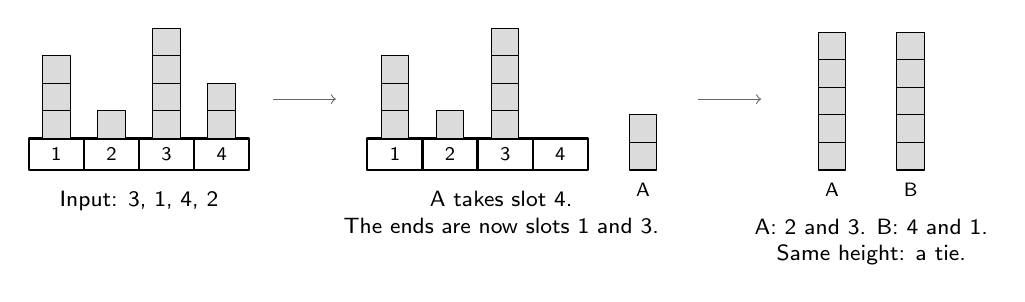
\begin{tikzpicture}[x=1mm,y=1mm,line join=round]
  % input
  \slots{0}{4}\tower{3.5}{4}{3}\tower{10.5}{4}{1}\tower{17.5}{4}{4}\tower{24.5}{4}{2}
  \node[font=\footnotesize,anchor=north] at (14,-1.5) {Input: 3, 1, 4, 2};
  \draw[->,black!60] (31,9) -- (39,9);
  % one move
  \slots{43}{4}\tower{46.5}{4}{3}\tower{53.5}{4}{1}\tower{60.5}{4}{4}
  \tower{78}{0}{2}\node[font=\scriptsize] at (78,-2.5) {A};
  \node[font=\footnotesize,anchor=north,align=center] at (60,-1.5) {A takes slot 4.\\ The ends are now slots 1 and 3.};
  \draw[->,black!60] (85,9) -- (93,9);
  % output
  \tower{102}{0}{5}\node[font=\scriptsize] at (102,-2.5) {A};
  \tower{112}{0}{5}\node[font=\scriptsize] at (112,-2.5) {B};
  \node[font=\footnotesize,anchor=north,align=center] at (107,-5) {A: 2 and 3. B: 4 and 1.\\ Same height: a tie.};
\end{tikzpicture}
\end{center}
The pictured game takes slots 4, 3, 1, 2. It is the worked record printed in grades 2--3 Problem 6, so that record will look familiar. The volunteer may choose differently; any finished game makes the point.

\textbf{A first hour, by band.} About 35--40 minutes at the tables; the timings are untested guesses. Each route ends with the grown-up's game, so that a child who comes once meets the colored strip; trim the plain-strip problems to get there, and save what is trimmed for a return visit. A table absorbed in plain play can stay there instead, and the grown-up's game opens the next visit. \emph{K--1}: Problem 1 with one or two rows; the first three rows of Problem 2; Problem 3; about five minutes of Problem 5's search, so that the grown-up's game answers a question the children already have; then Problem 6 for the last 10 minutes. Return visit: Problem 4 and the rest of Problem 2, then Problems 7 and 8. \emph{Grades 2--3}: Problem 1 with one or two rows; Problems 2 and 3; about five minutes of Problem 4's search; then Problem 5 with the adult for the last 10 minutes. Return visit: Problems 6--9. \emph{Grades 4--5}: Problems 1 and 2; about five minutes of Problem 3's search; then Problem 4 for the last 10 minutes. A quick group goes on to Problem 5; otherwise it opens the next visit. Return visits: Problems 5--9 (what colors decide), then Problems 10--11 (working backward), the deep end. Finishing every page is not the goal.

\head{Grades K--1: solutions and held hints}
Strips: plain strips of 4 and 3 (materials page 1) for Problems 1--5; colored strips of 4 and 6 (materials page 3) for Problems 6--8. Rows are listed left to right, then top to bottom, as printed. A child's own games may end differently from best play; any record that matches the stacks is right.

\pr{1}{1} With best play: 5, 2, 1, 4 is a first-player win 7--5 by taking the 5 (taking the 4 ties 6--6); 1, 5, 2, 3 is a first-player win 8--3 by taking the 3 (taking the 1 loses 4--7); 2, 4, 3, 1 is a tie 5--5 whatever the first move. Afterwards, if the table is curious: ``On which row would you rather go first?''

\pr{2}{2} The winning tower: 2, 1, 5, 3, slot 1 (the 2), 7--4. 3, 5, 1, 2, slot 4 (the 2), 7--4. 1, 1, 5, 2, slot 1 (the 1), 6--3. 2, 5, 1, 1, slot 4 (the 1), 6--3. 5, 1, 3, 2, slot 1 (the 5), 8--3. 2, 3, 1, 4, slot 4 (the 4), 7--3. The other first move loses the first five rows and only ties the last (5--5). Four of the six winning towers are the shorter end, so neither ``take the big one'' nor ``take the small one'' always works. A child's reason: ``If I take the 2, my partner has to take the 1 or the 3, and then I can reach the 5.'' ``However your partner plays'' means trying both of the partner's replies, which children can do by rebuilding the row. Hint: ``After you take it, which towers can your partner reach? Then which can you?'' Rows 3 and 4 are mirror images, a nice thing to notice. On a return visit, every winning tower here stands on the color with more cubes.

\pr{3}{3} 1, 5, 1: 2nd (2--5). 5, 1, 5: 1st (6--5). 1, 4, 2: 2nd (3--4). 3, 4, 2: 1st (5--4). 2, 5, 2: 2nd (4--5). A child's reason: ``Whoever goes first has to open up the big one.'' The row 3, 4, 2 shows a tall middle is not enough; stacking the two end towers (5) beside the middle (4) shows why. Hint: ``Who gets the middle tower? What does the other player get?'' Adult rule: the first player loses exactly when the middle is taller than both ends stacked together.

\pr{4}{4} Any row whose middle is taller than the two ends stacked together. With columns of five there are exactly ten: 1, 3, 1; 1, 4, 1; 1, 4, 2; 2, 4, 1; 1, 5, 1; 1, 5, 2; 2, 5, 1; 1, 5, 3; 3, 5, 1; 2, 5, 2. There are six boards, so nobody is expected to find all ten. Children check a drawing by building it and stacking the ends beside the middle, or by playing both first moves. Hint: ``How tall does the middle need to be?'' Extension: ``Can the middle be 3? Can it be 2?'' (3 only with 1, 3, 1; 2 never).

\pr{5}{5} No. The first player can always win or tie a row of four (all 625 rows with heights 1 to 5 checked; Theorem 1 proves it). Candidate rows will appear where the first player lost through an early mistake. Hint: ``Could the first player have done better starting at the other end?'' Do not announce that it is impossible; Problems 6 and 7 let them meet the plan that explains it. ``I tried lots and the first player always gets out of it'' is the right kind of evidence at this age.

\pr{6}{6} No: the grown-up wins all four by the card, 6--4, 6--4, 9--3 and 7--3, the same score whatever the team does. Let the children notice the color of the slots the grown-up's towers came from. Hint: ``Which slots did my towers stand on?'' Taking the taller end instead would lose the first row 4--6 and only tie the second 5--5, so follow the card even when its move looks wrong.

\pr{7}{7} Yes on every row, by the plan, and the child wins each one. 3, 1, 2, 5: blue 6 against red 5, start at slot 4 (the 5), 6--5 (best play gives 7--4). 2, 4, 1, 1: blue 5 against 3, start at slot 4 (the 1), 5--3; taking the taller 2 first loses 3--5 to a careful partner. 1, 3, 2, 1, 3, 1: red 6 against 5, start at slot 1, 6--5. 2, 1, 1, 3, 2, 2: blue 6 against 5, start at slot 6, 6--5. The totals are close on purpose. K--1 children compare them by counting the cubes on red slots and then on blue slots, or by building one copy stack per color from spare cubes and standing them side by side. Hint: ``Which color has more cubes? How could you check without taking the row apart?'' A child who wins without the plan can be asked how they chose.

\pr{8}{7} The K--1 deep end: winning needs looking two moves ahead. Rows 1 and 3. On 2, 1, 2, 3 take the 3 (slot 4) and win 5--3; on 4, 1, 2, 5 take the 5 (slot 4) and win 7--5. In both rows, starting at slot 1 only ties (4--4 and 6--6). On 1, 3, 4, 2 a careful partner holds you to a tie, 5--5, whatever you do. The careful partner's reply there: if the child takes the 2, the partner must take the 4 (taking the 1 loses 4--6); if the child takes the 1, either reply ties. The colors are equal in every row, so the plan promises only a tie. Hint: ``After you take that one, what can your partner reach?''

\head{Grades 2--3: solutions and held hints}
Strips: plain strips of 4 and 3 (materials page 1) for Problems 1--4; colored strips (materials page 3) of 6 and 8 for Problem 5, 6 for Problems 6 and 9, 4 for Problem 7 and 5 for Problem 8.
\pr{1}{1} 5, 2, 1, 4: 7--5 (take the 5; taking the 4 ties 6--6). 2, 6, 3, 4: 10--5 (take the 4; taking the 2 loses 6--9). 2, 4, 3, 1: 5--5. The table records the children's actual games; the two totals in a game always add to 12, 15 and 10, a check they can use. Afterwards: ``Was going first better on every row?''

\pr{2}{2} 2, 1, 5, 3: slot 1 (the 2), 7--4. 3, 6, 1, 2: slot 4 (the 2), 8--4. 2, 3, 1, 5: slot 4 (the 5), 8--3. 1, 4, 6, 2: slot 1 (the 1), 7--6. The other first move loses every row (5--6, 5--7, 5--6, 6--7). Row 3 is the one where the taller end wins, which breaks ``take the shorter end''. After the first move the partner has only two replies, so ``however your partner plays'' can be checked completely. Hint: ``If you take that one, what will your partner take? And then?'' Adult only: each winning tower stands on the color with more cubes; keep that for after Problem 5.

\pr{3}{2} second (2--5); first (6--5); second (5--6); first (5--4); no difference (5--5); second (5--6). The rule: compare the middle with the two ends added. Middle bigger, second wins; equal, no difference; smaller, first wins. A child's explanation with towers: if the middle is the tallest, whoever goes first must uncover it and the other player takes it, leaving the first player only the ends; if an end is at least as tall as the middle, the first player takes the taller end and comes out ahead. The row 3, 4, 2 refutes ``the tallest middle always loses'', and 2, 5, 3 is the tie. Hint: ``Who ends up with the middle tower, and what does the other player get?''

\pr{4}{3} No. All 1,296 rows with heights 1 to 6 are first-player wins or ties, and Theorem 1 proves it for any heights. Children will find rows that the first player lost through a careless first move. To check a candidate, try both first moves, play each out carefully, and add the tower the first player already took. Who wins the row of three that is left does not settle it: on 2, 4, 3, 1 (Problem 1's third row) the partner wins both rows of three that can be left, yet the first player, already holding the 2 or the 1, ties 5--5. Adult shortcut: on a row of three, the player to move collects both ends if the middle is the tallest, and otherwise the taller end plus the smaller of the other two. Leave the question open; Problems 5 and 6 supply the reason. Hint: ``After each first move, how many cubes does each player end up with?''

\pr{5}{4} Nobody beats the grown-up. 1, 2, 5, 1, 3, 2: red 9 against blue 5, start at slot 1 (the 1, not the taller 2), 9--5. 3, 1, 1, 4, 2, 2: blue 7 against red 6, start at slot 6, 7--6; best play would win 8--5 starting with the red 3, so the plan is safe rather than greedy. 1, 2, 3, 1, 2, 1, 3, 2: red 9 against 6, start at slot 1, 9--6. How the grown-up chooses: add each color, pick the larger, and always take the end tower of that color. Expect first guesses such as ``takes the bigger end''; the grown-up's first move on row 1 refutes it. Hint: ``Look at the slots where the grown-up's towers stood.''

\pr{6}{5} Red 6, blue 7, so take blue and start at slot 6. The partner can never make you take red. There are exactly four games, each 7--6: 6-1-2-3-4-5, 6-1-2-5-4-3, 6-5-4-1-2-3 and 6-5-4-3-2-1. The list is complete because your moves are forced and the partner has a real choice only with five towers left and with three left, two ways each. The six grids leave two spare. Why it always works: after each of your moves both ends are red, so the partner must take red and uncover a blue end. Hint: ``After your move, what color are the two end slots?'' Extension: with red instead there are again four games, and you lose 6--7 in each, so choosing the color matters.

\pr{7}{6} 2, 1, 2, 3: 5--3 (take the 3). 1, 3, 4, 2: 5--5. 4, 1, 2, 5: 7--5 (take the 5). 2, 4, 5, 3: 7--7. 3, 2, 4, 5: 8--6 (take the 5). The first player can win rows 1, 3 and 5; in each, starting at slot 1 only ties. Equal colors make the plan promise a tie, and looking ahead sometimes does better. Hint: ``What do you leave your partner to choose from?''

\pr{8}{7} 2, 1, 5, 1, 2: second wins 4--7, though red has 9 and blue 2. 4, 1, 1, 1, 4: first wins 6--5. 1, 4, 2, 4, 1: second wins 4--8. 1, 2, 4, 2, 1: tie 5--5. So the plan does not work: on a row of five both ends are red, and after the first move it is the second player who faces an even row. Hint: ``What colors are the two end slots on a row of five?'' Discretionary: ``Who gets to use the grown-up's plan here?''

\pr{9}{7} Possible: 1,974 of the 4,332 equal-color rows of six with heights 1 to 6 work. Examples: 2, 1, 2, 3, 1, 1 (start at slot 1, 6--4); 1, 1, 2, 1, 2, 3 (start at slot 6, 6--4); 1, 1, 4, 1, 2, 5 (10--4). Equal rows that only tie, useful when a child's claim needs testing: 1, 1, 1, 1, 3, 3 and 3, 1, 1, 1, 1, 3. Putting 1, 1 in front of a winning row from Problem 7 keeps the colors equal and works for all three of them (6--4, 10--4, 9--7). It worked on every equal-color winning row of four we checked by computer (heights 1 to 9), but it can fail on longer rows: 2, 1, 1, 2, 1, 1 wins 5--3, yet with 1, 1 in front it only ties 5--5, so a child's claim that it always works still needs a reason. Children test an invention by having a partner try hard against it from both first moves; the adult can confirm with the table of grades 4--5 Problem 11. Hint: ``Which rows in Problem 7 could the first player win? Could one of them grow?''

\head{Grades 4--5: solutions and held hints}
Strips: plain strips of 4 and 3 (materials page 1) for Problems 1--3; colored strips (materials page 3) of 6 and 8 for Problem 4, 4 for Problem 6 and 5 for Problems 7--9; plain strips of 5 and 6 (materials page 2) for Problems 10 and 11.
\pr{1}{1} 2, 1, 5, 3: first by 3 (7--4). 1, 4, 6, 2: first by 1 (7--6). 2, 4, 3, 1: tie (5--5). 6, 2, 1, 5: first by 2 (8--6, take the 6; taking the 5 ties 7--7). Every first move leaves a row of three: work out what each player collects on it and add the tower already taken. Problem 2's rule says who wins the row of three, not the row of four: on 6, 2, 1, 5 the partner wins both rows of three that can be left (2, 1, 5 by 6--2 and 6, 2, 1 by 7--2), yet the first player, already holding the 6, wins 8--6. Hint: ``After each first move, how many cubes does each player end up with?''

\pr{2}{1} 1, 5, 1: 2--5. 5, 1, 5: 6--5. 2, 6, 3: 5--6. 3, 4, 2: 5--4. 2, 5, 3: 5--5. 6, 1, 2: 7--2. The rule and its proof are in Theorem 2. Watch for ``the biggest middle loses'' (3, 4, 2 refutes it) and for explanations that consider only one first move. Discretionary: ``Does your explanation cover a row whose tallest tower is at an end?''

\pr{3}{2} No; all 1,296 rows checked. A long search is evidence, not proof. Children may conjecture ``the first player never loses on four''; let it stand as a conjecture until Problem 5. Hint: ``Could the first player have started at the other end?''

\pr{4}{3} The same rows as grades 2--3 Problem 5, written as numbers: the grown-up wins 9--5, 7--6 and 9--6, playing as on the grown-up's card. Hint: ``Which slots did my towers stand on?''

\pr{5}{3} A complete explanation: the number of towers is even, so the two ends have different colors. I take an end of my color. Now both ends are the other color, so you must take one of yours, which leaves exactly one end of my color for me. So I take every tower of my color and you take every tower of yours, and I chose the color with at least as many cubes. Watch for explanations that show ``I can always take my color'' but not ``you can never take mine'', or that skip why the ends start out different. Discretionary: ``Where does your argument use `even'?''

\pr{6}{4} 2, 1, 2, 3: first by 2 (5--3, take the 3). 1, 3, 4, 2: tie (5--5). 4, 1, 2, 5: first by 2 (7--5, take the 5). 2, 4, 5, 3: tie (7--7). 3, 1, 1, 3: tie (4--4). 4, 2, 1, 3: first by 2 (6--4, take the 4; taking the 3 ties 5--5). The plan promises a tie; taking towers of both colors sometimes wins. Hint: ``What does each first move leave your partner?''

\pr{7}{4} The second player wins all four: 4--8, 5--8, 6--9, 5--6. Both ends of a row of five are red, so the first player takes a red tower. The second player then faces an even row with every blue tower still there and can take them all, getting at least the blue total, which is more than the red total, the most the first player can get. Hint: ``After the first move, who is in the grown-up's position?''

\pr{8}{5} 4, 1, 1, 1, 4: first by 1 (6--5). 1, 2, 4, 2, 1: tie (5--5). 2, 1, 5, 1, 2: second by 3 (4--7). 4, 2, 1, 2, 4: first by 1 (7--6). 4, 1, 6, 2, 3: second by 2 (7--9). More red than blue decides nothing. Discretionary: ``Why doesn't Problem 7's explanation work for the first player here?''

\pr{9}{5} No. As in Problem 7, the second player can take every blue tower, which is half of all the cubes, so the first player gets at most half. A tie can happen: 1, 2, 2, 2, 1 ties 4--4.

\pr{10}{6} 3, 1, 4, 1, 5: take the 5, tie 7--7 (taking the 3 loses 5--9). 2, 1, 2, 5, 3: take the 2 at slot 1, first by 1 (7--6); taking the taller 3 loses 6--7. 5, 2, 6, 1, 3: take the 5, second wins by 1 (8--9); taking the 3 loses 6--11. ``Best'' on a losing row means losing by less, as the first page defines. Each first move leaves a row of four, which is Problem 1's kind of work: this is working backward. If both players always take the taller end, row 2 ends 6--7, so greed costs the first player the win. Hint: ``Which row of four is left after each first move, and who goes first on it?''

\pr{11}{6} From the bottom row up: 2, 3, 6, 2, 1, 4; then 3, 6, 6, 2, 4; then 8, 5, 7, 5; then 8, 7, 8; then 7, 9; top 11. The rule children can find: a box is the total of its row minus the smaller of the two boxes beneath it, because after you take an end your partner becomes the player to move on one of those rows. The top box is 11 of 18 cubes, so the first player wins 11--7 by taking the 4, which leaves 2, 3, 6, 2, 1 (worth 7 to the partner); taking the 2 leaves 3, 6, 2, 1, 4 (worth 9), a 9--9 tie. The color totals are 9 and 9, another equal-color win as in Problem 6. Hint: ``What is the most you can be sure of from one tower? From two?'' Extension: build the table for a row from Problem 10, or for a child's own row of six.

\head{Sources and what to record}
Peter Winkler, \emph{Mathematical Puzzles: A Connoisseur's Collection} (A K Peters, 2004), the puzzle ``Coins in a Row'', to which Peterson attributes the even-row strategy. Not consulted directly; page not checked. Ivars Peterson, ``Coins in a Row'', \emph{Science News} (Math Trek), May 13, 2005, \url{https://www.sciencenews.org/article/coins-row-0}, consulted October 25, 2026: reports Winkler's odd/even-position strategy for an even number of coins, the penny--nickel--penny and nickel--penny--nickel examples (our 1, 5, 1 and 5, 1, 5), and that no one has ``worked out an optimal strategy that works for any number of coins''. Alexander Bogomolny, ``A Game With Coins'', cut-the-knot, \url{https://www.cut-the-knot.org/Curriculum/Games/Coins.shtml}, consulted October 25, 2026: the same parity strategy guaranteeing at least a draw, the 1, 5, 1 and 5, 1, 5 examples, and a citation of Winkler. The backward recurrence is standard interval dynamic programming. The outline links this theme to Weeks 7 and 8 (working backward, copying the opponent), Week 1e (copying on symmetric boards) and atlas AP-21 (a backward table of best scores); those links are the outline's and were not rechecked here. The towers, strips, rows and problem sequence are ours, and every printed score was recomputed for this guide by a script (\texttt{check\_guide.py}).

\textbf{What to record.} Which problems each table reached and in what order; rows children invented and what they claimed about them; what children said the grown-up was doing before anyone named colors; whether K--1 children compared color totals by counting or by stacking; whether the adult could run the plan without slowing the game; and any moment an adult chose a child's move. Keep observations separate from guesses about why they happened. Note which pages remain, so returning children can resume.

\end{document}
